% !TEX root = presentation.tex
%LTeX: language=de-CH

% \section{Einleitung}

\begin{frame}
	\frametitle{Karte}
	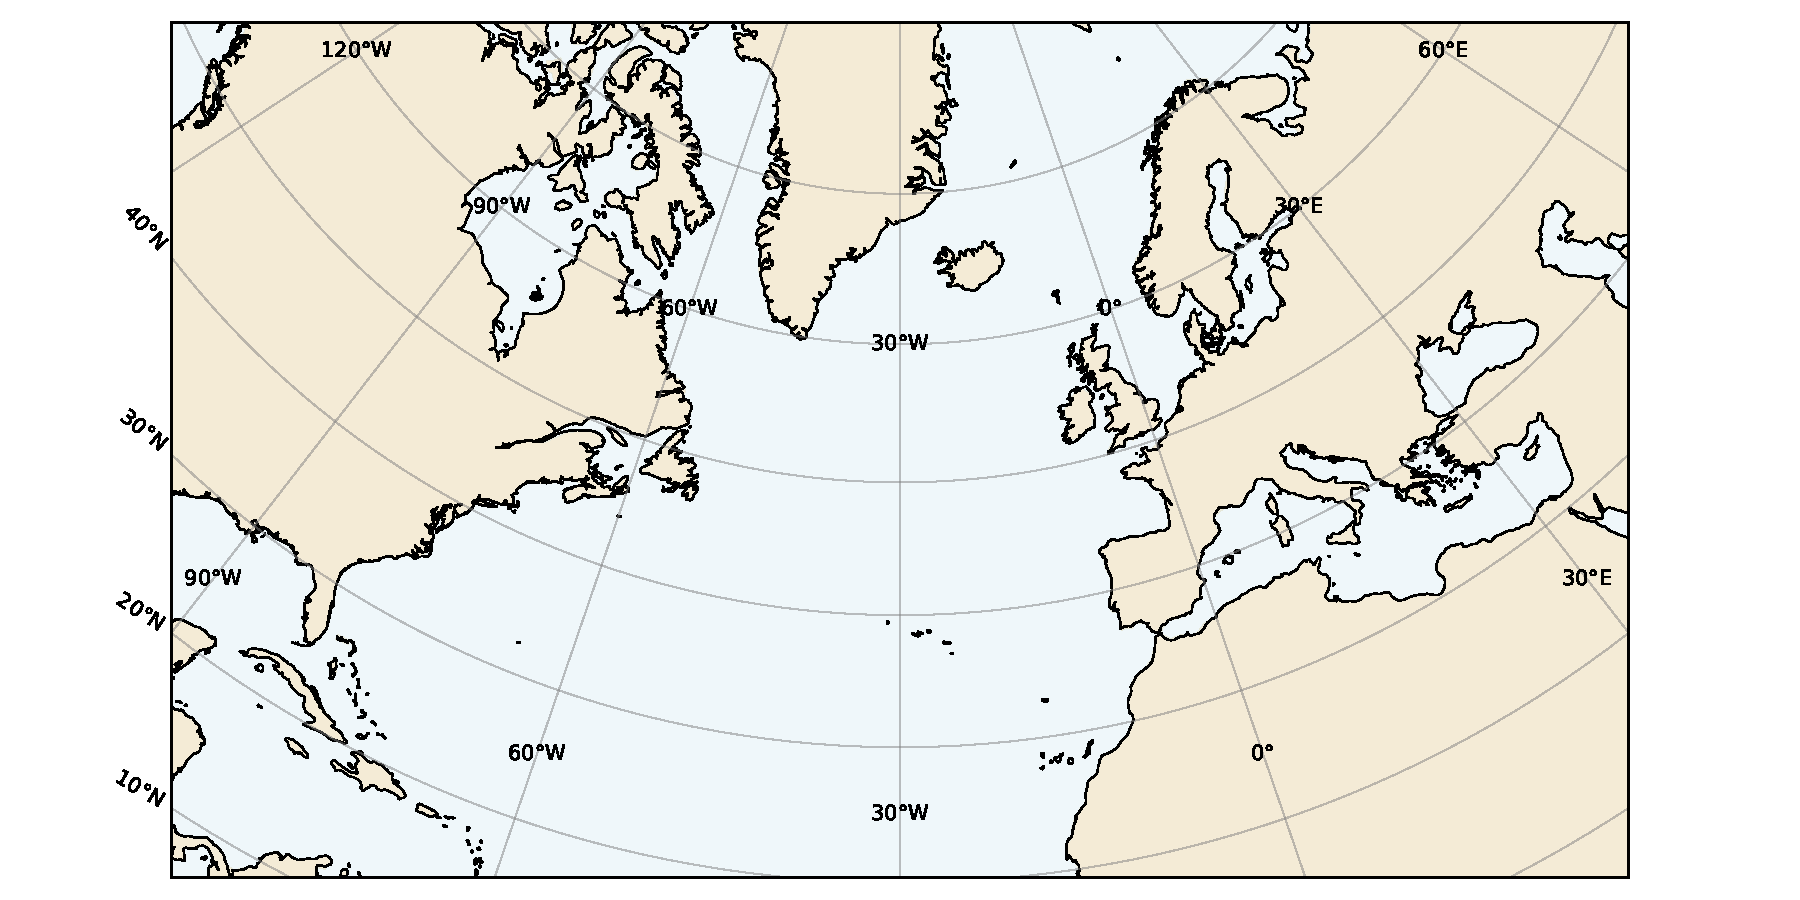
\includegraphics[width=\textwidth]{../images/weather/map.pdf}
\end{frame}

\begin{frame}
	\frametitle{Forecast: 01-May-2025 at 00:00, Level 850 hPa}
	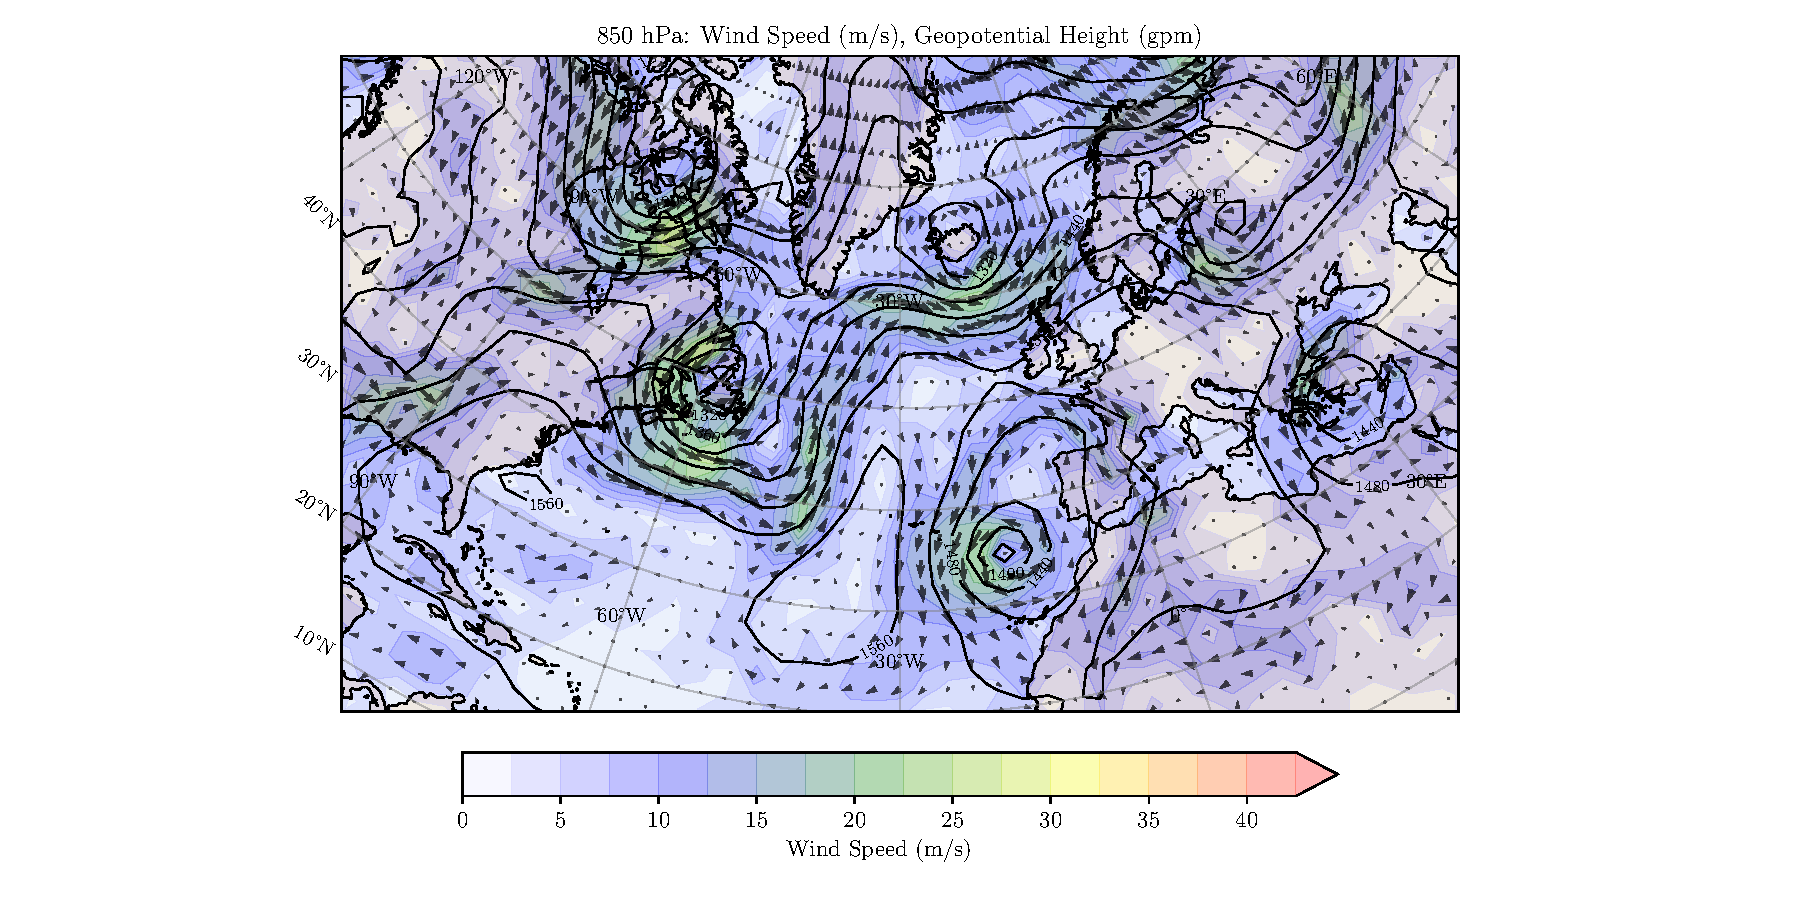
\includegraphics[width=\textwidth]{../images/weather/data_2025_5_1_00:00_850.pdf}
\end{frame}



\begin{frame}{ERA5-Analyse: Jetstream am Mai 2025}
	\begin{itemize}
		\item Datenquelle: \textbf{ERA5 Reanalysis} (ECMWF) via CDS API
		\item Abfrageparameter:
		      \begin{itemize}
			      \item Druckniveau: \textbf{500 hPa} (obere Troposphäre, Jetstream-Niveau)
			      \item Variablen: Geopotential, \( u \)- und \( v \)-Windkomponente
		      \end{itemize}
		\item Visualisierung:
		      \begin{itemize}
			      \item Farbkarte: Windgeschwindigkeit (m/s)
			      \item Linien: Geopotentielle Höhe (gpm)
			      \item Pfeile: Windvektoren
		      \end{itemize}
	\end{itemize}
\end{frame}

\begin{frame}
	\frametitle{Forecast: 01-May-2025 at 00:00, Level 500 hPa}
	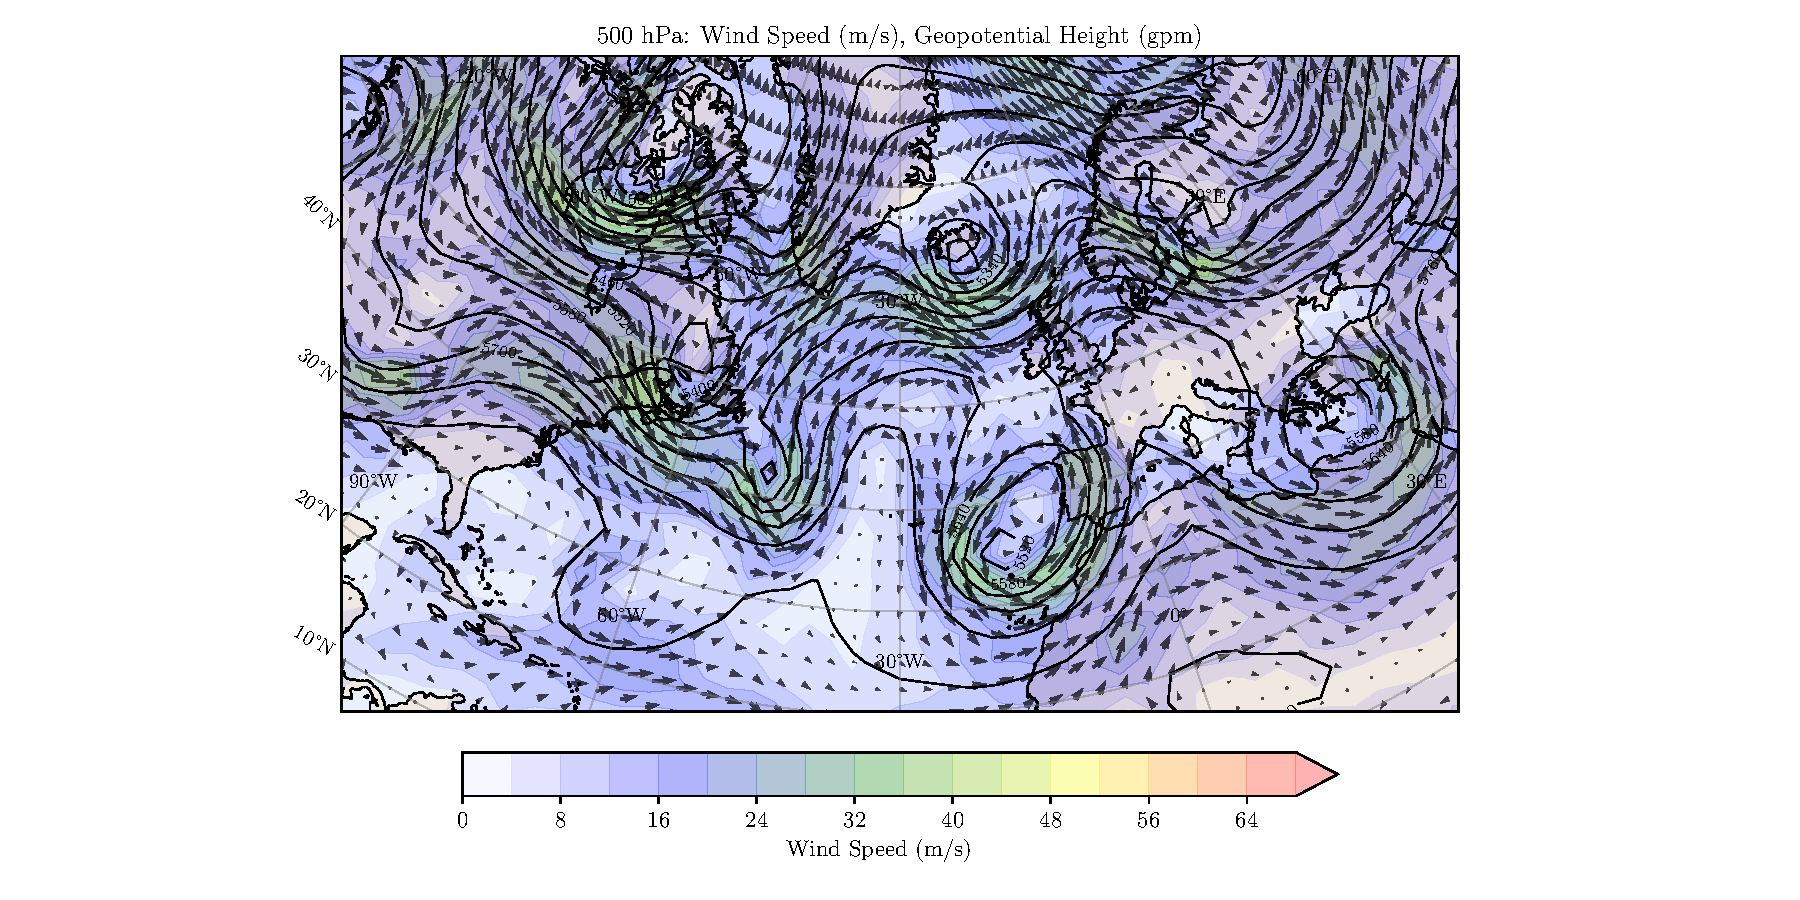
\includegraphics[width=\textwidth]{../images/weather/data_2025_5_1_00:00_500.pdf}
\end{frame}
\begin{frame}
	\frametitle{Forecast: 01-May-2025 at 00:00, Level 200 hPa}
	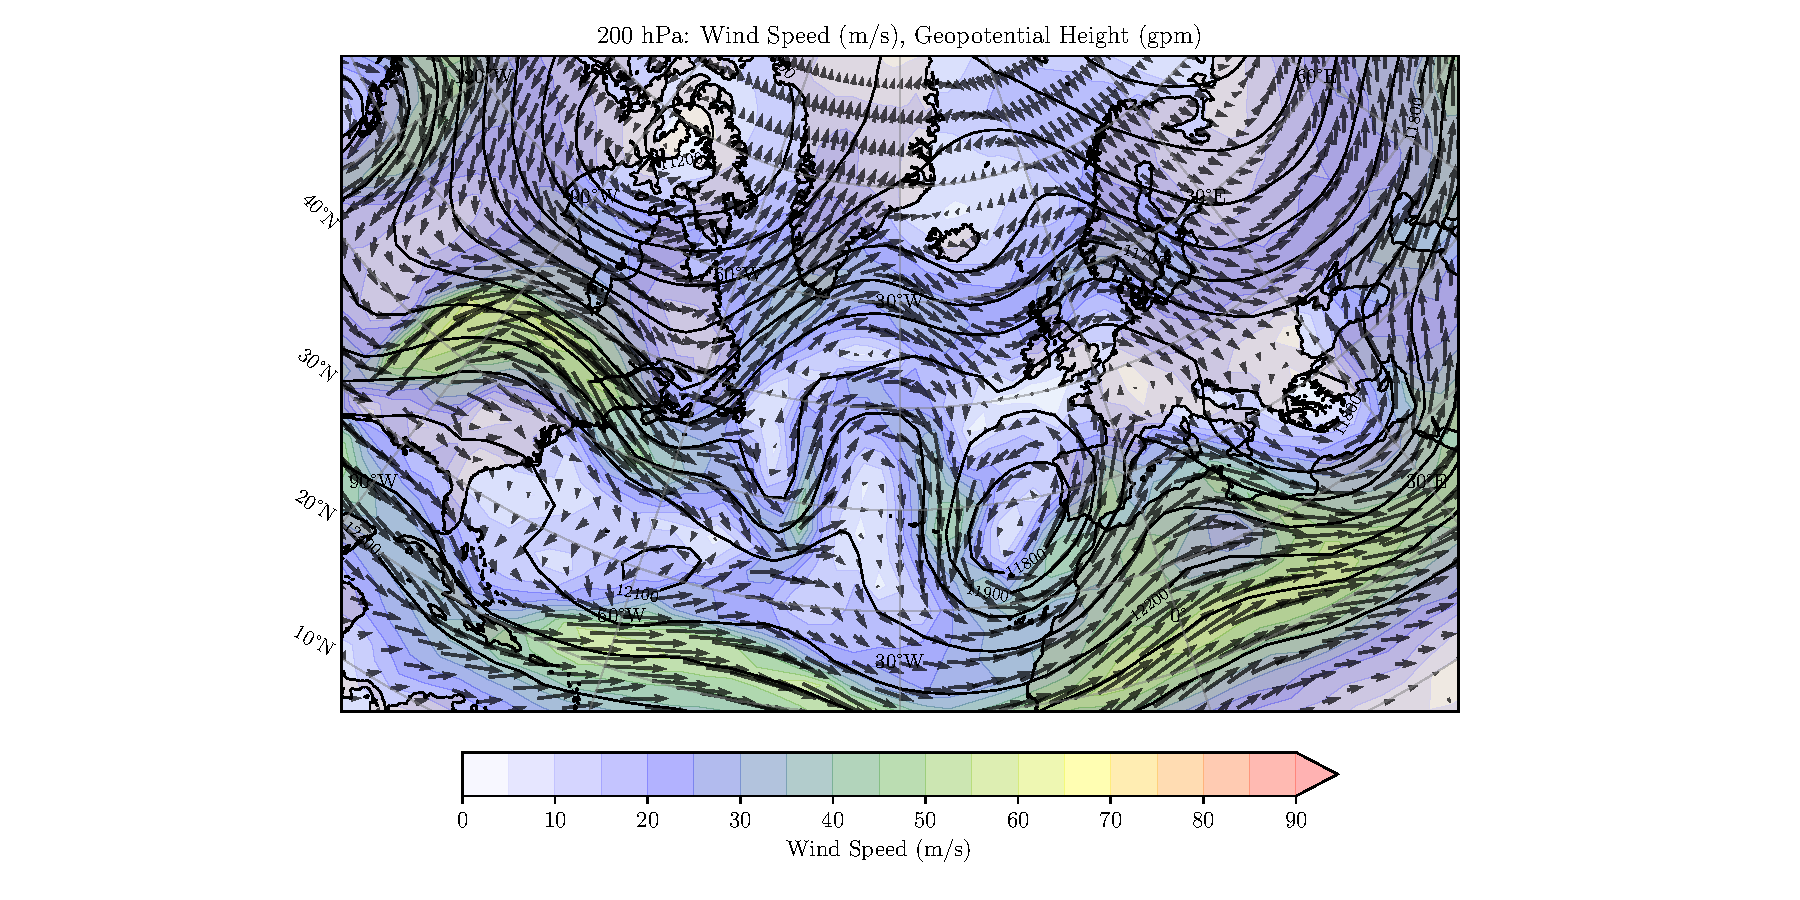
\includegraphics[width=\textwidth]{../images/weather/data_2025_5_1_00:00_200.pdf}
\end{frame}

% \begin{frame}{Warum 850, 500 und 200 hPa?}
% 	\vspace{-0.3cm}
% 	\begin{itemize}
% 		\item Standard-Druckniveaus in der Meteorologie
% 		\item Repräsentieren typische Höhenbereiche der Troposphäre mit jeweils spezifischer dynamischer Bedeutung
% 	\end{itemize}

% 	\vspace{0.2cm}
% 	\begin{table}[h]
% 		\centering
% 		\begin{tabular}{|c|c|p{7cm}|}
% 			\hline
% 			\textbf{Niveau} & \textbf{Höhe (ca.)} & \textbf{Bedeutung}                                                                    \\
% 			\hline
% 			850 hPa         & ~1.5 km             & Untere Troposphäre: Temperatur, Feuchtigkeit, Hebung, Konvektion, Bodeninversion      \\
% 			\hline
% 			500 hPa         & ~5.5 km             & Mittlere Troposphäre: Vorticity, Tröge/Rücken, synoptische Dynamik, Luftmassengrenzen \\
% 			\hline
% 			200 hPa         & ~12 km              & Obere Troposphäre: Jetstream, Divergenzfelder, Rossby-Wellen, barokline Kopplung      \\
% 			\hline
% 		\end{tabular}
% 	\end{table}
% \end{frame}




% In your document body:

\foreach \level in {500} {
		\foreach \day in {1,...,10} {
				\foreach \time in {00:00,12:00} {
						\begin{frame}
							\frametitle{Forecast: \day-May-2025 at \time, Level \level hPa}
							\includegraphics[width=\textwidth]{../images/weather/data_2025_5_\day_\time_\level.pdf}
						\end{frame}
					}
			}
	}



% In your document body:
\foreach \level in {500} {
		\foreach \day in {1,...,10} {
				\foreach \time in {00:00,12:00} {
						\begin{frame}[plain]
							\frametitle{Forecast: \day-May-2025 at \time, Level \level hPa}
							\begin{center}
								\includegraphics[width=0.5\textwidth]{../images/weather/data_2025_5_\day_\time_\level_polar.pdf}
							\end{center}
						\end{frame}
					}
			}
	}
